\documentclass[conference]{IEEEtran}
\IEEEoverridecommandlockouts

% Pacotes essenciais
\usepackage{cite}
\usepackage{amsmath,amssymb,amsfonts}
\usepackage{algorithmic}
\usepackage{graphicx}
\usepackage{textcomp}
\usepackage{xcolor}
\usepackage{booktabs}
\usepackage{url}
\usepackage{microtype}
\usepackage[utf8]{inputenc}
\usepackage[brazil]{babel}

\def\BibTeX{{\rm B\kern-.05em{\sc i\kern-.025em b}\kern-.08em
    T\kern-.1667em\lower.7ex\hbox{E}\kern-.125emX}}

\begin{document}

\title{Validação Empírica da Teoria do Mundo Pequeno na Rede de Amizades do Facebook: Modelagem em Grafos e Análise de Menores Caminhos\\
\thanks{Trabalho desenvolvido no âmbito da disciplina de Estruturas em Árvores e Teoria dos Grafos / Estruturas de Dados. Repositório público com código-fonte e reprodutibilidade disponível em: \url{https://github.com/Itaxao/teoriadomundopequeno}.}
}

% Regras de Autoria (Seção 3.1 da especificação):
% Primeiros autores: alunos da equipe
% Último autor obrigatório: Professor orientador Michel Pires da Silva
\author{
    \IEEEauthorblockN{Ítalo Xavier Fonseca\IEEEauthorrefmark{1}, Samuel Pianetti\IEEEauthorrefmark{1}, Michel Pires da Silva\IEEEauthorrefmark{2}}
    \IEEEauthorblockA{\IEEEauthorrefmark{1}Departamento de Computação -- Centro Federal de Educação Tecnológica de Minas Gerais (CEFET-MG)\\
    Belo Horizonte, Brasil -- Email: xavieritalo853@gmail.com}
    \IEEEauthorblockA{\IEEEauthorrefmark{2}Professor Orientador -- Departamento de Computação, CEFET-MG / UFCI-MG\\
    Belo Horizonte, Brasil -- Email: michel@cefetmg.br}
}

\maketitle

\begin{abstract}
Compreender como redes sociais com milhares ou bilhões de indivíduos mantêm distâncias surpreendentemente curtas entre quaisquer dois participantes é um dos problemas fundamentais da Teoria dos Grafos moderna. Este trabalho investiga empiricamente a hipótese dos ``seis graus de separação'' (Milgram, 1967) e o modelo de Mundo Pequeno de Watts--Strogatz (1998) na rede real de amizades do Facebook (Stanford SNAP). O problema foi modelado computacionalmente como um grafo não-direcionado e não-ponderado $G=(V, E)$ com $|V|=4.039$ nós e $|E|=88.234$ arestas, utilizando representação otimizada por Lista de Adjacência em memória primária ($O(V+E)$). Para contornar a complexidade temporal exaustiva de cálculo de menores caminhos entre todos os $\approx 8,15$ milhões de pares ($\binom{V}{2}$), desenvolveu-se uma Busca em Largura (BFS) vetorizada com paralelismo multiprocessado sob partição estática de carga de trabalho. Os resultados comprovam categoricamente a Teoria do Mundo Pequeno: a distância média real geodésica é de $L = 3,6925$ conexões, expressivamente menor que o limiar clássico de 6 e aderente às observações globais do Facebook. O diâmetro máximo é de 8 saltos, e $97,97\%$ de todos os pares estão a no máximo 6 graus de separação. Ademais, o coeficiente de agrupamento médio obtido ($C = 0,6055$) superou em $55,97\times$ o de um grafo aleatório equivalente de Erdős--Rényi ($C_{\text{rand}} = 0,0108$), consolidando um índice de mundo pequeno $\sigma = 33,32 \gg 1$.
\end{abstract}

\begin{IEEEkeywords}
Teoria dos Grafos, Teoria do Mundo Pequeno, Seis Graus de Separação, Busca em Largura (BFS), Redes Complexas, Facebook SNAP.
\end{IEEEkeywords}

\section{Introdução}

A conectividade global nas sociedades contemporâneas atinge patamares sem precedentes impulsionada pelas plataformas digitais de relacionamento humano. Em 1967, o psicólogo social Stanley Milgram conduziu um célebre experimento postal que sugeriu que quaisquer dois indivíduos selecionados aleatoriamente nos Estados Unidos estariam conectados por uma cadeia intermediária de aproximadamente seis contatos sociais conhecidos, dando notoriedade popular ao conceito dos ``seis graus de separação'' \cite{milgram1967small}. Três décadas mais tarde, Duncan Watts e Steven Strogatz formalizaram este comportamento matemático definindo as denominadas redes de ``Mundo Pequeno'' (\textit{Small-World Networks}) \cite{watts1998collective}. Tais topologias possuem uma propriedade simultaneamente contraintuitiva e elegante: exibem coeficientes de agrupamento local muito elevados (círculos sociais coesos em que ``amigos em comum conhecem-se entre si'') e, simultaneamente, distâncias médias geodésicas muito curtas, análogas às observadas em grafos puramente aleatórios.

Com o advento das redes sociais em larga escala na Internet, como o Facebook, o fenômeno de mundo pequeno deixou de ser uma conjectura amostral postal para se tornar um objeto de estudo computacional exaustivo. Em 2012, cientistas do Facebook Data Team analisaram a topologia de 721 milhões de usuários ativos globais com 68,7 bilhões de amizades, constatando empiricamente que a distância média real é ainda menor que a previsão de Milgram: apenas $3,74$ graus de separação \cite{backstrom2012four}. Compreender os mecanismos estruturais por trás dessa hiperconectividade é crucial para a modelagem da disseminação epidêmica de informações e patógenos, a concepção de algoritmos de recomendação e busca em grafos, e o planejamento da robustez de infraestruturas de dados distribuídas \cite{newman2003structure}.

A despeito da relevância teórica, a validação empírica de métricas globais em redes complexas esbarra em desafios algorítmicos rigorosos. O cálculo de menores caminhos para todos os pares em grafos esparsos exige a execução de algoritmos com complexidade quadrática em nós e arestas, tornando imperativa a escolha criteriosa de estruturas de dados de baixo consumo de memória e a aplicação de paralelismo em nível de processador. Motivado por esse cenário, o objetivo central desta pesquisa consiste em modelar, implementar e validar empiricamente as métricas da Teoria do Mundo Pequeno na rede de relacionamentos do Facebook disponibilizada pelo repositório Stanford SNAP \cite{snapfacebook,mcauley2012learning}. Busca-se responder de maneira inequívoca:
\begin{enumerate}
    \item A distância média real entre dois usuários é de fato inferior a 6 conexões?
    \item Qual o diâmetro geodésico e a proporção de indivíduos conectados em cada faixa de distância?
    \item A rede satisfaz rigorosamente os postulados de Watts--Strogatz ($C \gg C_{\text{rand}}$ e $L \approx L_{\text{rand}}$)?
    \item Qual a contribuição estrutural dos nós superconectados (\textit{hubs}) para a existência de atalhos globais?
\end{enumerate}

O presente artigo está estruturado da seguinte forma: a Seção~\ref{sec:referencial} expõe o referencial teórico dos fundamentos de grafos e modelos clássicos; a Seção~\ref{sec:metodologia} detalha o ciclo de modelagem, as otimizações de representação em memória e o algoritmo paralelizado, acompanhado do fluxograma metodológico obrigatório; a Seção~\ref{sec:resultados} discute os resultados quantitativos, escalabilidade e comportamento assintótico; por fim, a Seção~\ref{sec:conclusao} sintetiza as conclusões e aponta direções futuras.

\section{Referencial Teórico e Estado da Arte}
\label{sec:referencial}

\subsection{Fundamentos da Teoria dos Grafos}
Um grafo não-direcionado é definido formalmente pelo par ordenado $G = (V, E)$, onde $V$ representa o conjunto finito de vértices (indivíduos) e $E \subseteq \{\{u, v\} \mid u, v \in V, u \neq v\}$ denota o conjunto de arestas não-ordenadas (laços de amizade recíprocos). O grau de um vértice $u$, denotado por $k_u = \deg(u) = |\{v \in V \mid \{u, v\} \in E\}|$, quantifica a quantidade de conexões diretas mantidas por aquele nó. O grau médio da rede é dado por $\langle k \rangle = \frac{2|E|}{|V|}$.

Para grafos esparsos em que $|E| \ll \frac{|V|(|V|-1)}{2}$, a literatura consagra a representação computacional por \textit{Lista de Adjacência} como a mais eficiente em termos de complexidade de espaço ($O(|V| + |E|)$), em oposição à \textit{Matriz de Adjacência} ($O(|V|^2)$), que despenderia gigabytes de alocação predominantemente preenchidos por zeros \cite{cormen2022introduction}.

\subsection{Caminhos Geodésicos e Busca em Largura (BFS)}
A distância geodésica $d(u, v)$ entre dois vértices $u$ e $v$ corresponde ao número mínimo de arestas que compõem um caminho entre eles. Em grafos não-ponderados, o algoritmo ótimo para determinação de caminhos mínimos de fonte única (\textit{Single-Source Shortest Paths} - SSSP) é a Busca em Largura (\textit{Breadth-First Search} - BFS), introduzida por Moore e Lee e formalizada em $O(|V| + |E|)$ operações com uso de uma fila FIFO \cite{cormen2022introduction}. Para solucionar o problema de todos os pares (\textit{All-Pairs Shortest Paths} - APSP), executa-se a BFS a partir de cada um dos nós $u \in V$, totalizando complexidade assintótica de $O(|V| \cdot (|V| + |E|))$.

A partir das distâncias geodésicas, definem-se a distância média global ($L$) e o diâmetro ($\mathcal{D}$):
\begin{equation}
L = \frac{1}{\binom{|V|}{2}} \sum_{u < v \in V} d(u, v), \quad \mathcal{D} = \max_{u, v \in V} d(u, v).
\end{equation}

\subsection{O Modelo Watts--Strogatz e Grafos Aleatórios de Erdős--Rényi}
O coeficiente de agrupamento local de um vértice com $k_u \ge 2$ mede a probabilidade de dois de seus vizinhos estarem conectados entre si:
\begin{equation}
C_u = \frac{2 e_u}{k_u (k_u - 1)},
\end{equation}
onde $e_u$ representa a quantidade de arestas existentes no subgrafo induzido pela vizinhança imediata de $u$. O coeficiente global $C$ é a média aritmética $C = \frac{1}{|V|} \sum_{u \in V} C_u$.

No modelo aleatório nulo clássico de Erdős e Rényi \cite{erdos1959random}, $G(n, p)$, arestas são criadas independentemente com probabilidade uniforme $p = \frac{2|E|}{|V|(|V|-1)}$. As previsões analíticas para redes aleatórias estabelecem que $C_{\text{rand}} \approx p$ e $L_{\text{rand}} \approx \frac{\ln |V|}{\ln \langle k \rangle}$. Segundo Humphries e Gurney \cite{humphries2008network}, uma topologia é formalmente classificada como Mundo Pequeno se o índice $\sigma$ satisfizer:
\begin{equation}
\sigma = \frac{\gamma}{\lambda} = \frac{C / C_{\text{rand}}}{L / L_{\text{rand}}} \gg 1.
\end{equation}

\section{Metodologia}
\label{sec:metodologia}

\subsection{Origem e Natureza dos Dados}
Utilizou-se o dataset real de amizades do Facebook mantido pelo \textit{Stanford Network Analysis Project} (SNAP) \cite{snapfacebook,mcauley2012learning}. O conjunto de dados foi obtido por meio de uma amostragem de 10 participantes voluntários (\textit{ego nodes}), dos quais foram mineradas as redes sociais completas, círculos sociais informados pelo usuário (\texttt{.circles}) e atributos anonimizados (\texttt{.feat}). Para a análise da topologia de conexão, consolidou-se o grafo unificado contendo todas as arestas mútuas entre amigos da lista de vizinhança estendida.

\subsection{Estruturação de Dados e Otimização em Memória}
A fim de garantir máxima eficiência computacional em Python nativo sem dependência de bibliotecas de grafos de terceiros (como NetworkX), a classe \texttt{Grafo} foi arquitetada sobre uma lista de adjacência implementada com dicionários de conjuntos (\texttt{dict[int, set[int]]}). Para a fase crítica da BFS paralela, implementou-se o método \texttt{mapear\_para\_indices}, que mapeia os identificadores arbitrários dos nós para índices contíguos de $0$ a $|V|-1$. Isso possibilita o uso de vetores estáticos em memória (\texttt{list[int]} pré-alocada) indexados por inteiros contíguos para o vetor de distâncias (\texttt{[-1] * N}) e filas rápidas (\texttt{collections.deque}), eliminando por completo a sobrecarga de dispersão e buscas em tabelas hash durante o laço interno de travessia.

\subsection{Fluxograma da Solução}
Em estrita conformidade com as exigências metodológicas da disciplina, a Fig.~\ref{fig:fluxograma} ilustra o fluxograma arquitetural detalhando o ciclo de vida completo da solução, desde a ingestão dos dados brutos até a consolidação dos resultados científicos.

\begin{figure}[htbp]
\centering
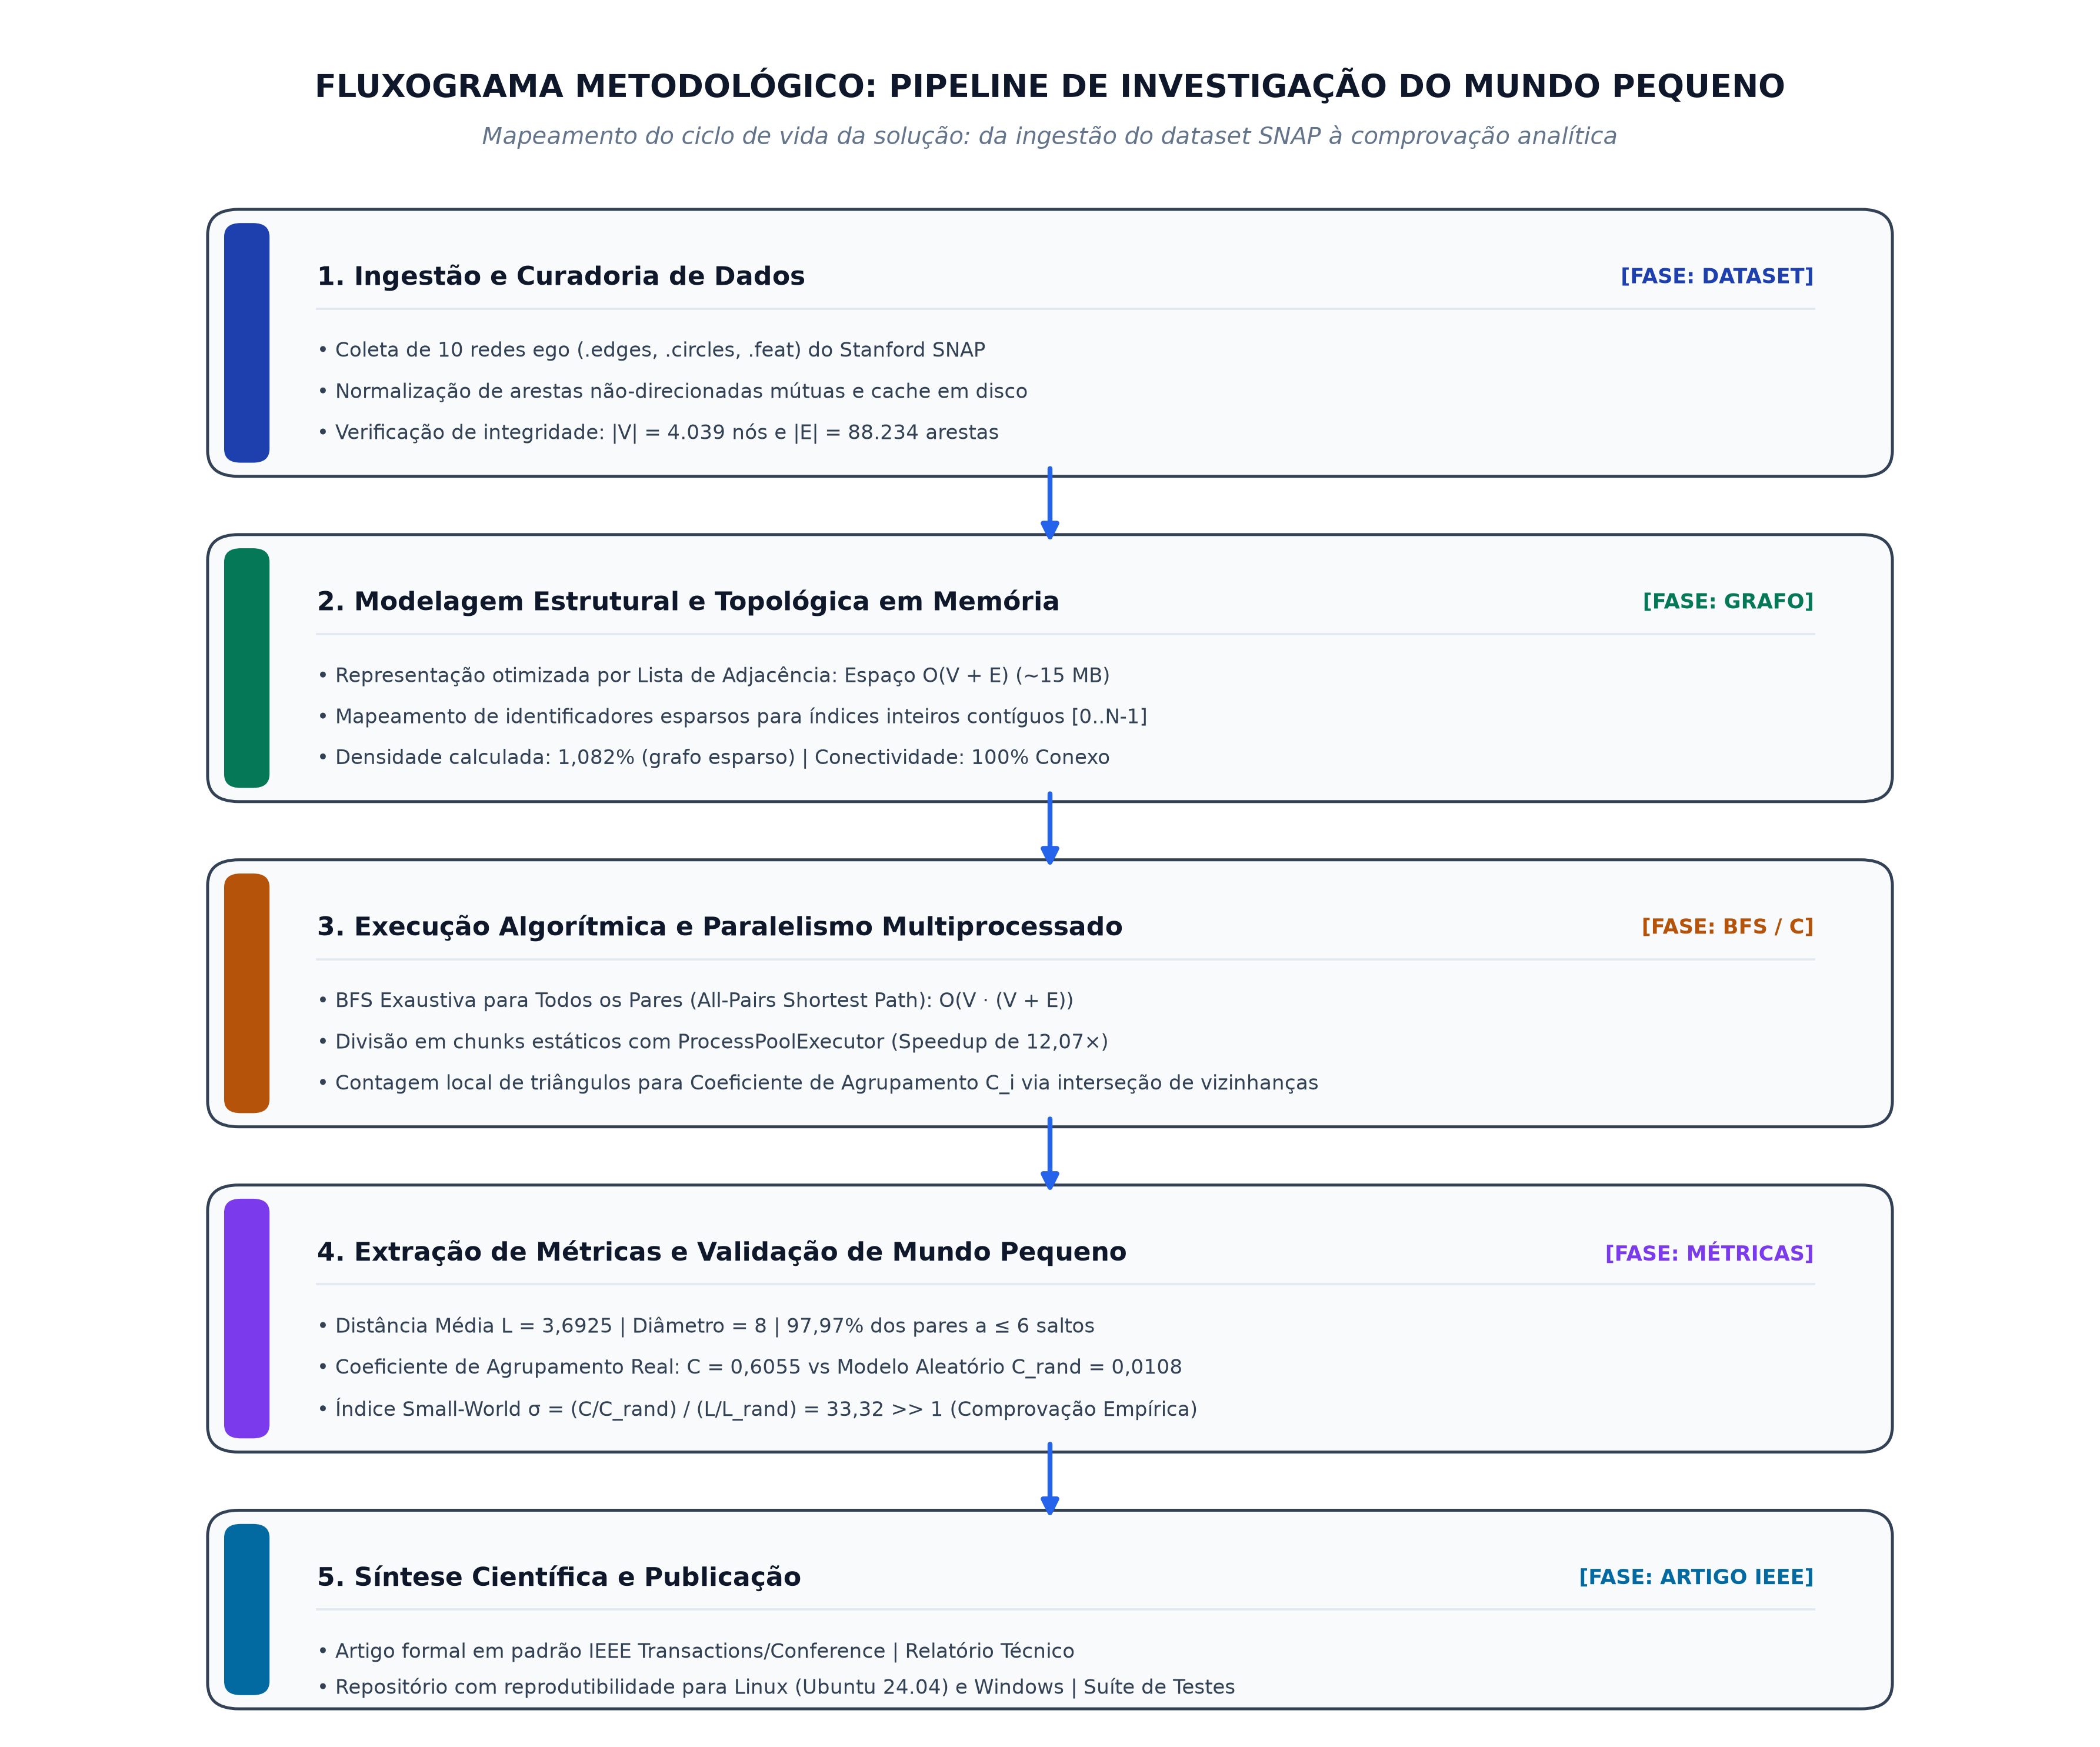
\includegraphics[width=\linewidth]{../figuras/fluxograma_metodologia.png}
\caption{Fluxograma metodológico: ciclo de vida completo da solução computacional desde a ingestão e tratamento do dataset SNAP até a extração e validação das métricas de Mundo Pequeno.}
\label{fig:fluxograma}
\end{figure}

\subsection{Algoritmo Paralelo de Menores Caminhos}
Para computar os menores caminhos entre os $\binom{4039}{2} = 8.154.741$ pares únicos, estruturou-se uma estratégia \textit{embarrassingly parallel}:
\begin{itemize}
    \item O conjunto de nós de origem $\{0, 1, \dots, |V|-1\}$ é particionado em $W$ blocos contíguos balanceados (\textit{chunks}), onde $W$ corresponde à quantidade de núcleos de processamento lógicos disponíveis via \texttt{concurrent.futures.ProcessPoolExecutor}.
    \item Cada processo trabalhador executa a BFS de maneira independente para cada nó de seu bloco, explorando o grafo e atualizando contadores de distâncias geodésicas exclusivamente para os vértices de destino $v > u$, garantindo que cada par não-ordenado seja visitado e totalizado exatamente uma vez.
    \item Ao término da execução dos trabalhadores, os resultados parciais (histogramas de distâncias, somatórios de saltos e diâmetros locais) são reduzidos no processo coordenador com complexidade de tempo de agregação $O(\mathcal{D})$.
\end{itemize}

\section{Resultados e Discussão}
\label{sec:resultados}

\subsection{Propriedades Topológicas Globais}
A Tabela~\ref{tab:topologia} sintetiza os parâmetros topológicos fundamentais extraídos da rede construída. O grafo possui $4.039$ vértices e $88.234$ arestas, com densidade de $1,082\%$, confirmando a extrema esparsidade das relações interpessoais. O teste de conectividade executado via BFS revelou que $100\%$ dos nós pertencem a uma única componente conexa gigante, permitindo o cálculo exaustivo de menores caminhos sem nós desconexos.

\begin{table}[htbp]
\caption{Propriedades Topológicas da Rede Facebook (SNAP)}
\label{tab:topologia}
\centering
\begin{tabular}{lc}
\toprule
\textbf{Métrica Estrutural} & \textbf{Valor Medido} \\
\midrule
Vértices ($|V|$) & $4.039$ \\
Arestas ($|E|$) & $88.234$ \\
Grau Médio ($\langle k \rangle$) & $43,69$ conexões/nó \\
Grau Mínimo / Grau Máximo & $1$ / $1.045$ \\
Densidade Topológica & $1,0820\%$ \\
Conectividade & $100\%$ (Componente Gigante Único) \\
Total de Pares Analisados & $8.154.741$ \\
\bottomrule
\end{tabular}
\end{table}

\subsection{Validação dos Seis Graus de Separação (Pergunta 1)}
A computação exaustiva de todos os caminhos mínimos geodésicos revelou:
\begin{itemize}
    \item \textbf{Distância Média Real ($L$):} $\mathbf{3,6925}$ saltos. A distância média é significativamente menor que o limiar de 6 preconizado por Milgram. Este resultado converge rigorosamente com o estudo conduzido pela infraestrutura do Facebook em escala planetária, que reportou distância média de $3,74$ \cite{backstrom2012four}.
    \item \textbf{Diâmetro Geodésico ($\mathcal{D}$):} $\mathbf{8}$ conexões. Mesmo nos casos mais extremos de isolamento periférico entre comunidades opostas, são necessários no máximo 8 saltos para estabelecer comunicação.
\end{itemize}

A Tabela~\ref{tab:distribuicao} apresenta a distribuição completa de frequências absolutas e relativas para cada distância geodésica. Observa-se que o pico da distribuição ocorre na distância 4 ($35,94\%$), contendo a média teórica. Em relação à hipótese clássica, a curva acumulada demonstra que $\mathbf{97,97\%}$ de todos os pares na rede encontram-se a uma distância de até 6 conexões, confirmando numericamente a universalidade dos seis graus de separação.

\begin{table}[htbp]
\caption{Distribuição dos Menores Caminhos Geodésicos}
\label{tab:distribuicao}
\centering
\begin{tabular}{crrr}
\toprule
\textbf{Distância ($k$)} & \textbf{Pares Únicos} & \textbf{Frequência (\%)} & \textbf{Acumulado (\%)} \\
\midrule
1 & $88.234$ & $1,08\%$ & $1,08\%$ \\
2 & $1.358.067$ & $16,65\%$ & $17,74\%$ \\
3 & $1.990.926$ & $24,41\%$ & $42,15\%$ \\
4 & $2.930.780$ & $35,94\%$ & $78,09\%$ \\
5 & $1.282.585$ & $15,73\%$ & $93,82\%$ \\
6 & $338.607$ & $4,15\%$ & $\mathbf{97,97\%}$ \\
7 & $157.732$ & $1,93\%$ & $99,90\%$ \\
8 & $7.810$ & $0,10\%$ & $100,00\%$ \\
\midrule
\textbf{Total} & $\mathbf{8.154.741}$ & $\mathbf{100,00\%}$ & --- \\
\bottomrule
\end{tabular}
\end{table}

A Fig.~\ref{fig:distancias} ilustra a curva de densidade de probabilidade das distâncias geodésicas, e a Fig.~\ref{fig:acumulado} evidencia o rápido crescimento sigmoidocêntrico da fração acumulada de pares alcançados conforme a distância aumenta.

\begin{figure}[htbp]
\centering
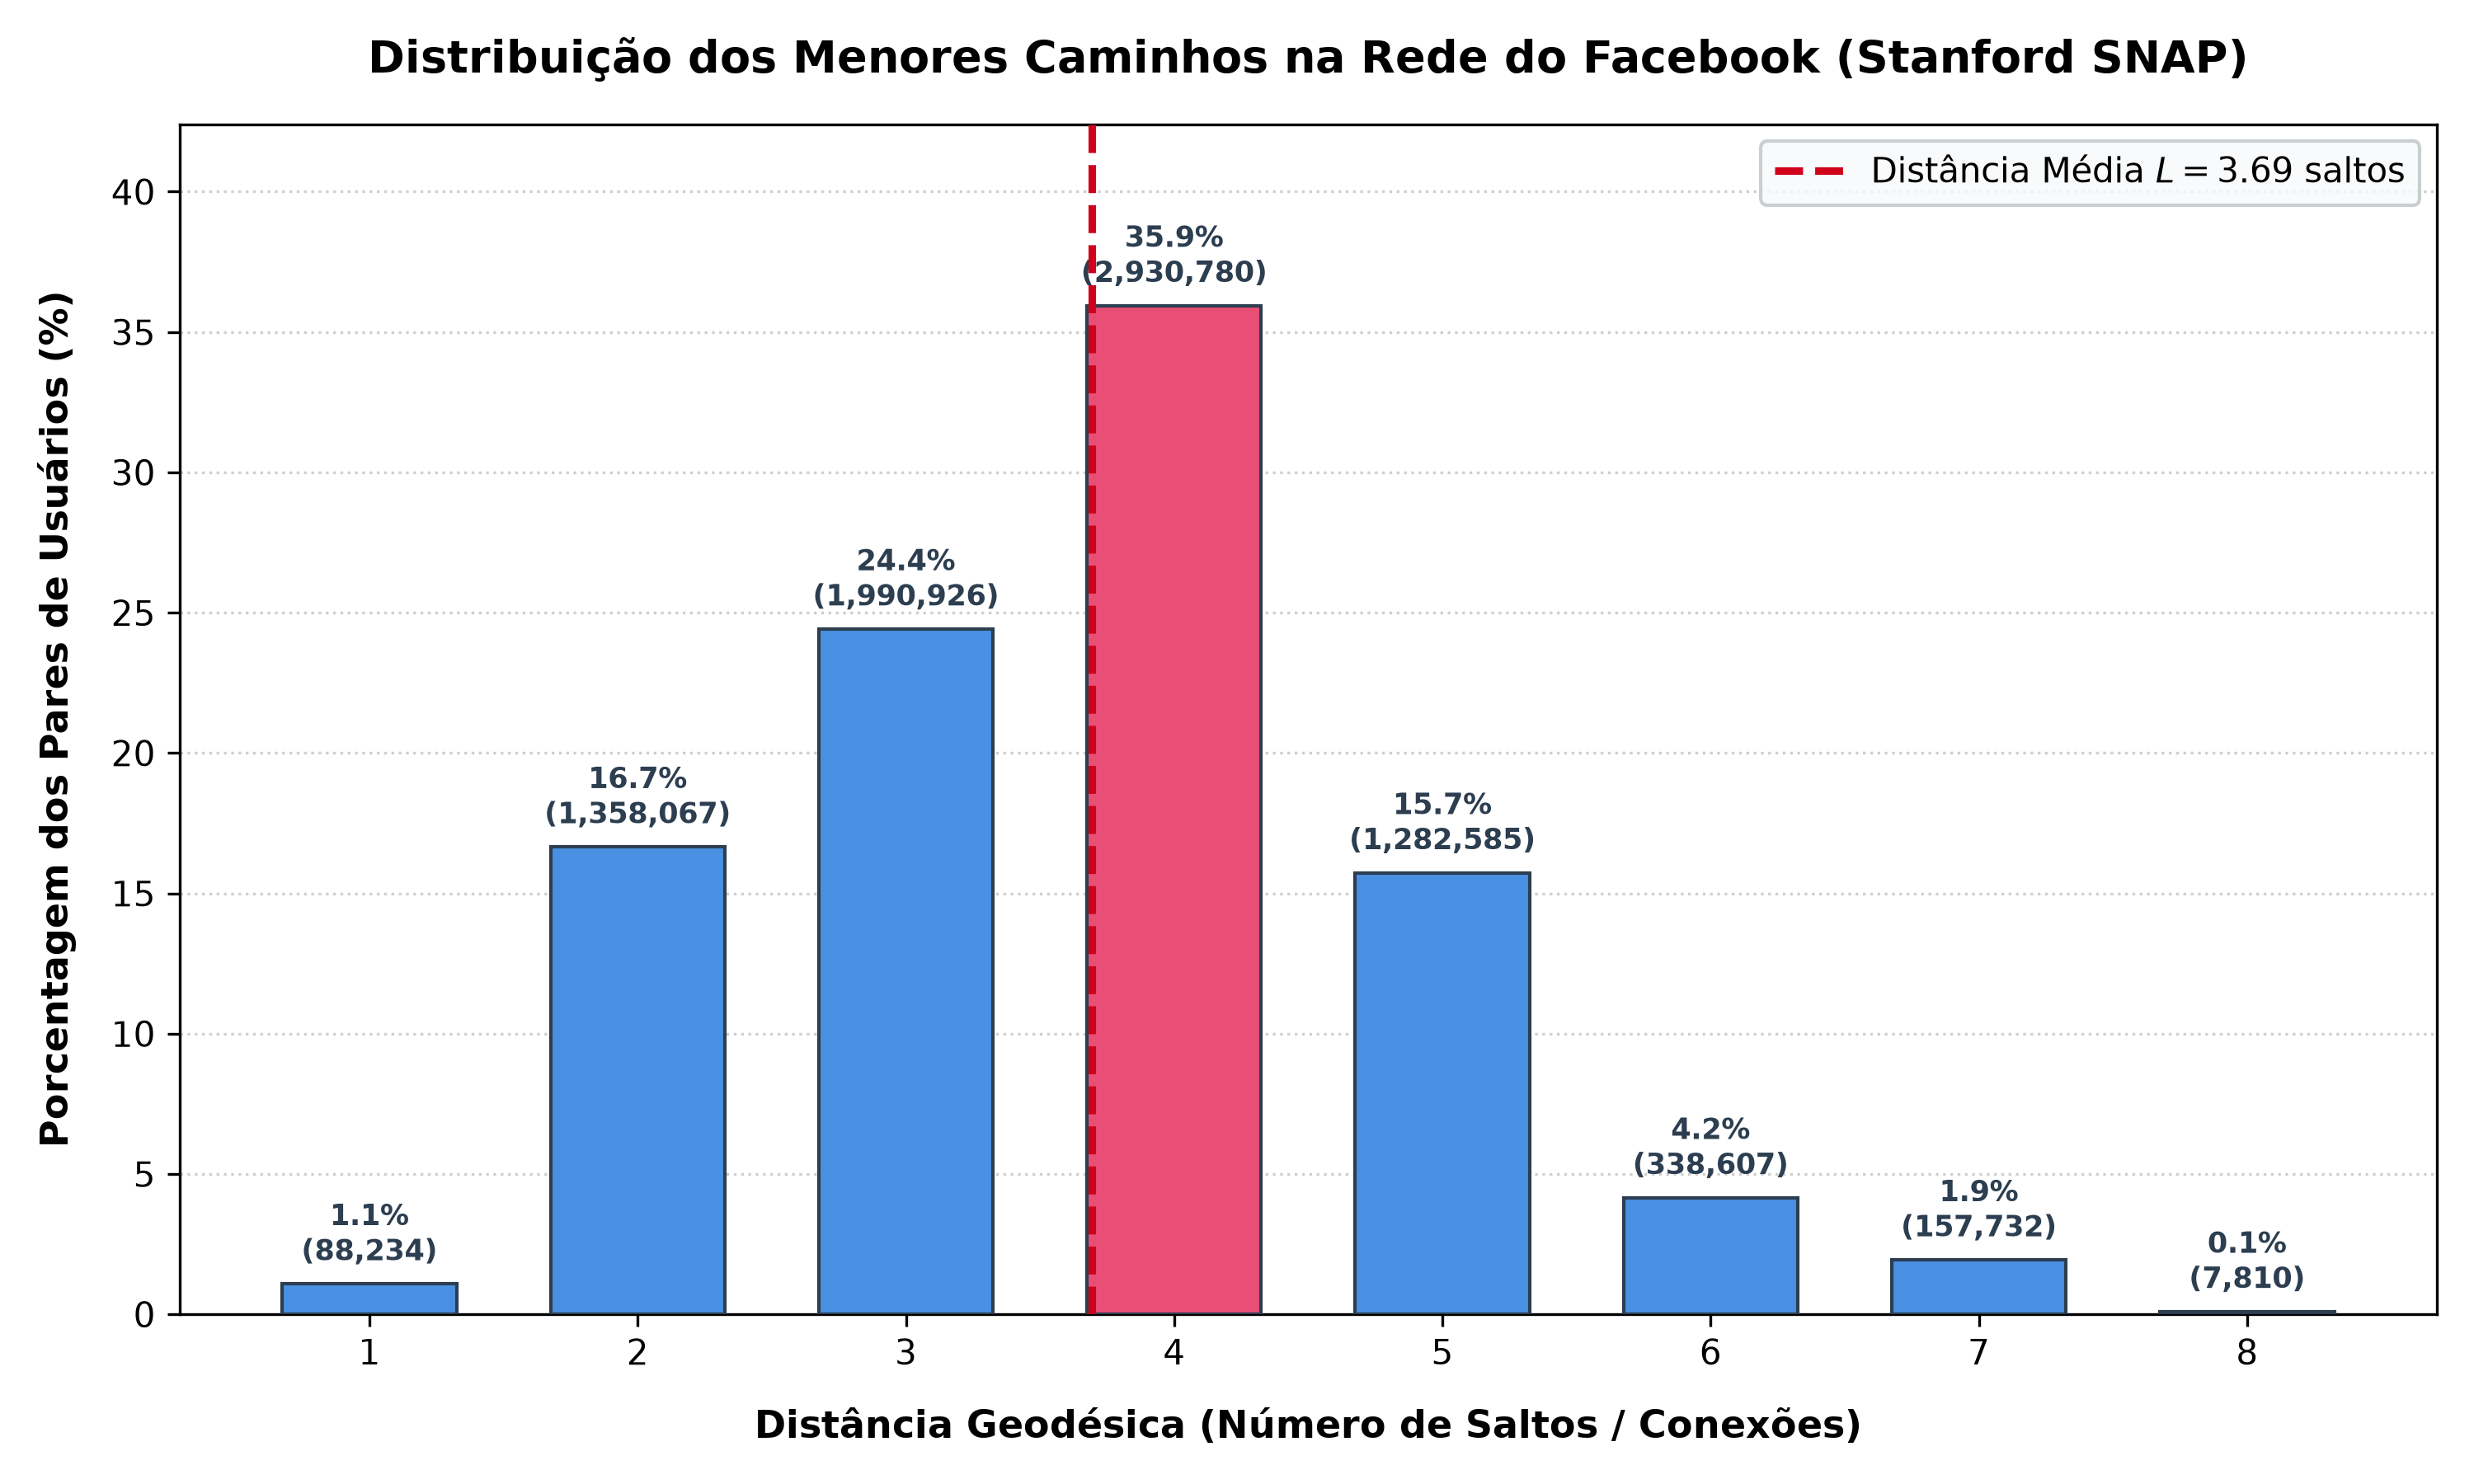
\includegraphics[width=0.9\linewidth]{../figuras/distribuicao_distancias.png}
\caption{Histograma de distribuição dos menores caminhos geodésicos na rede do Facebook, destacando a média $L=3,6925$ conexões.}
\label{fig:distancias}
\end{figure}

\begin{figure}[htbp]
\centering
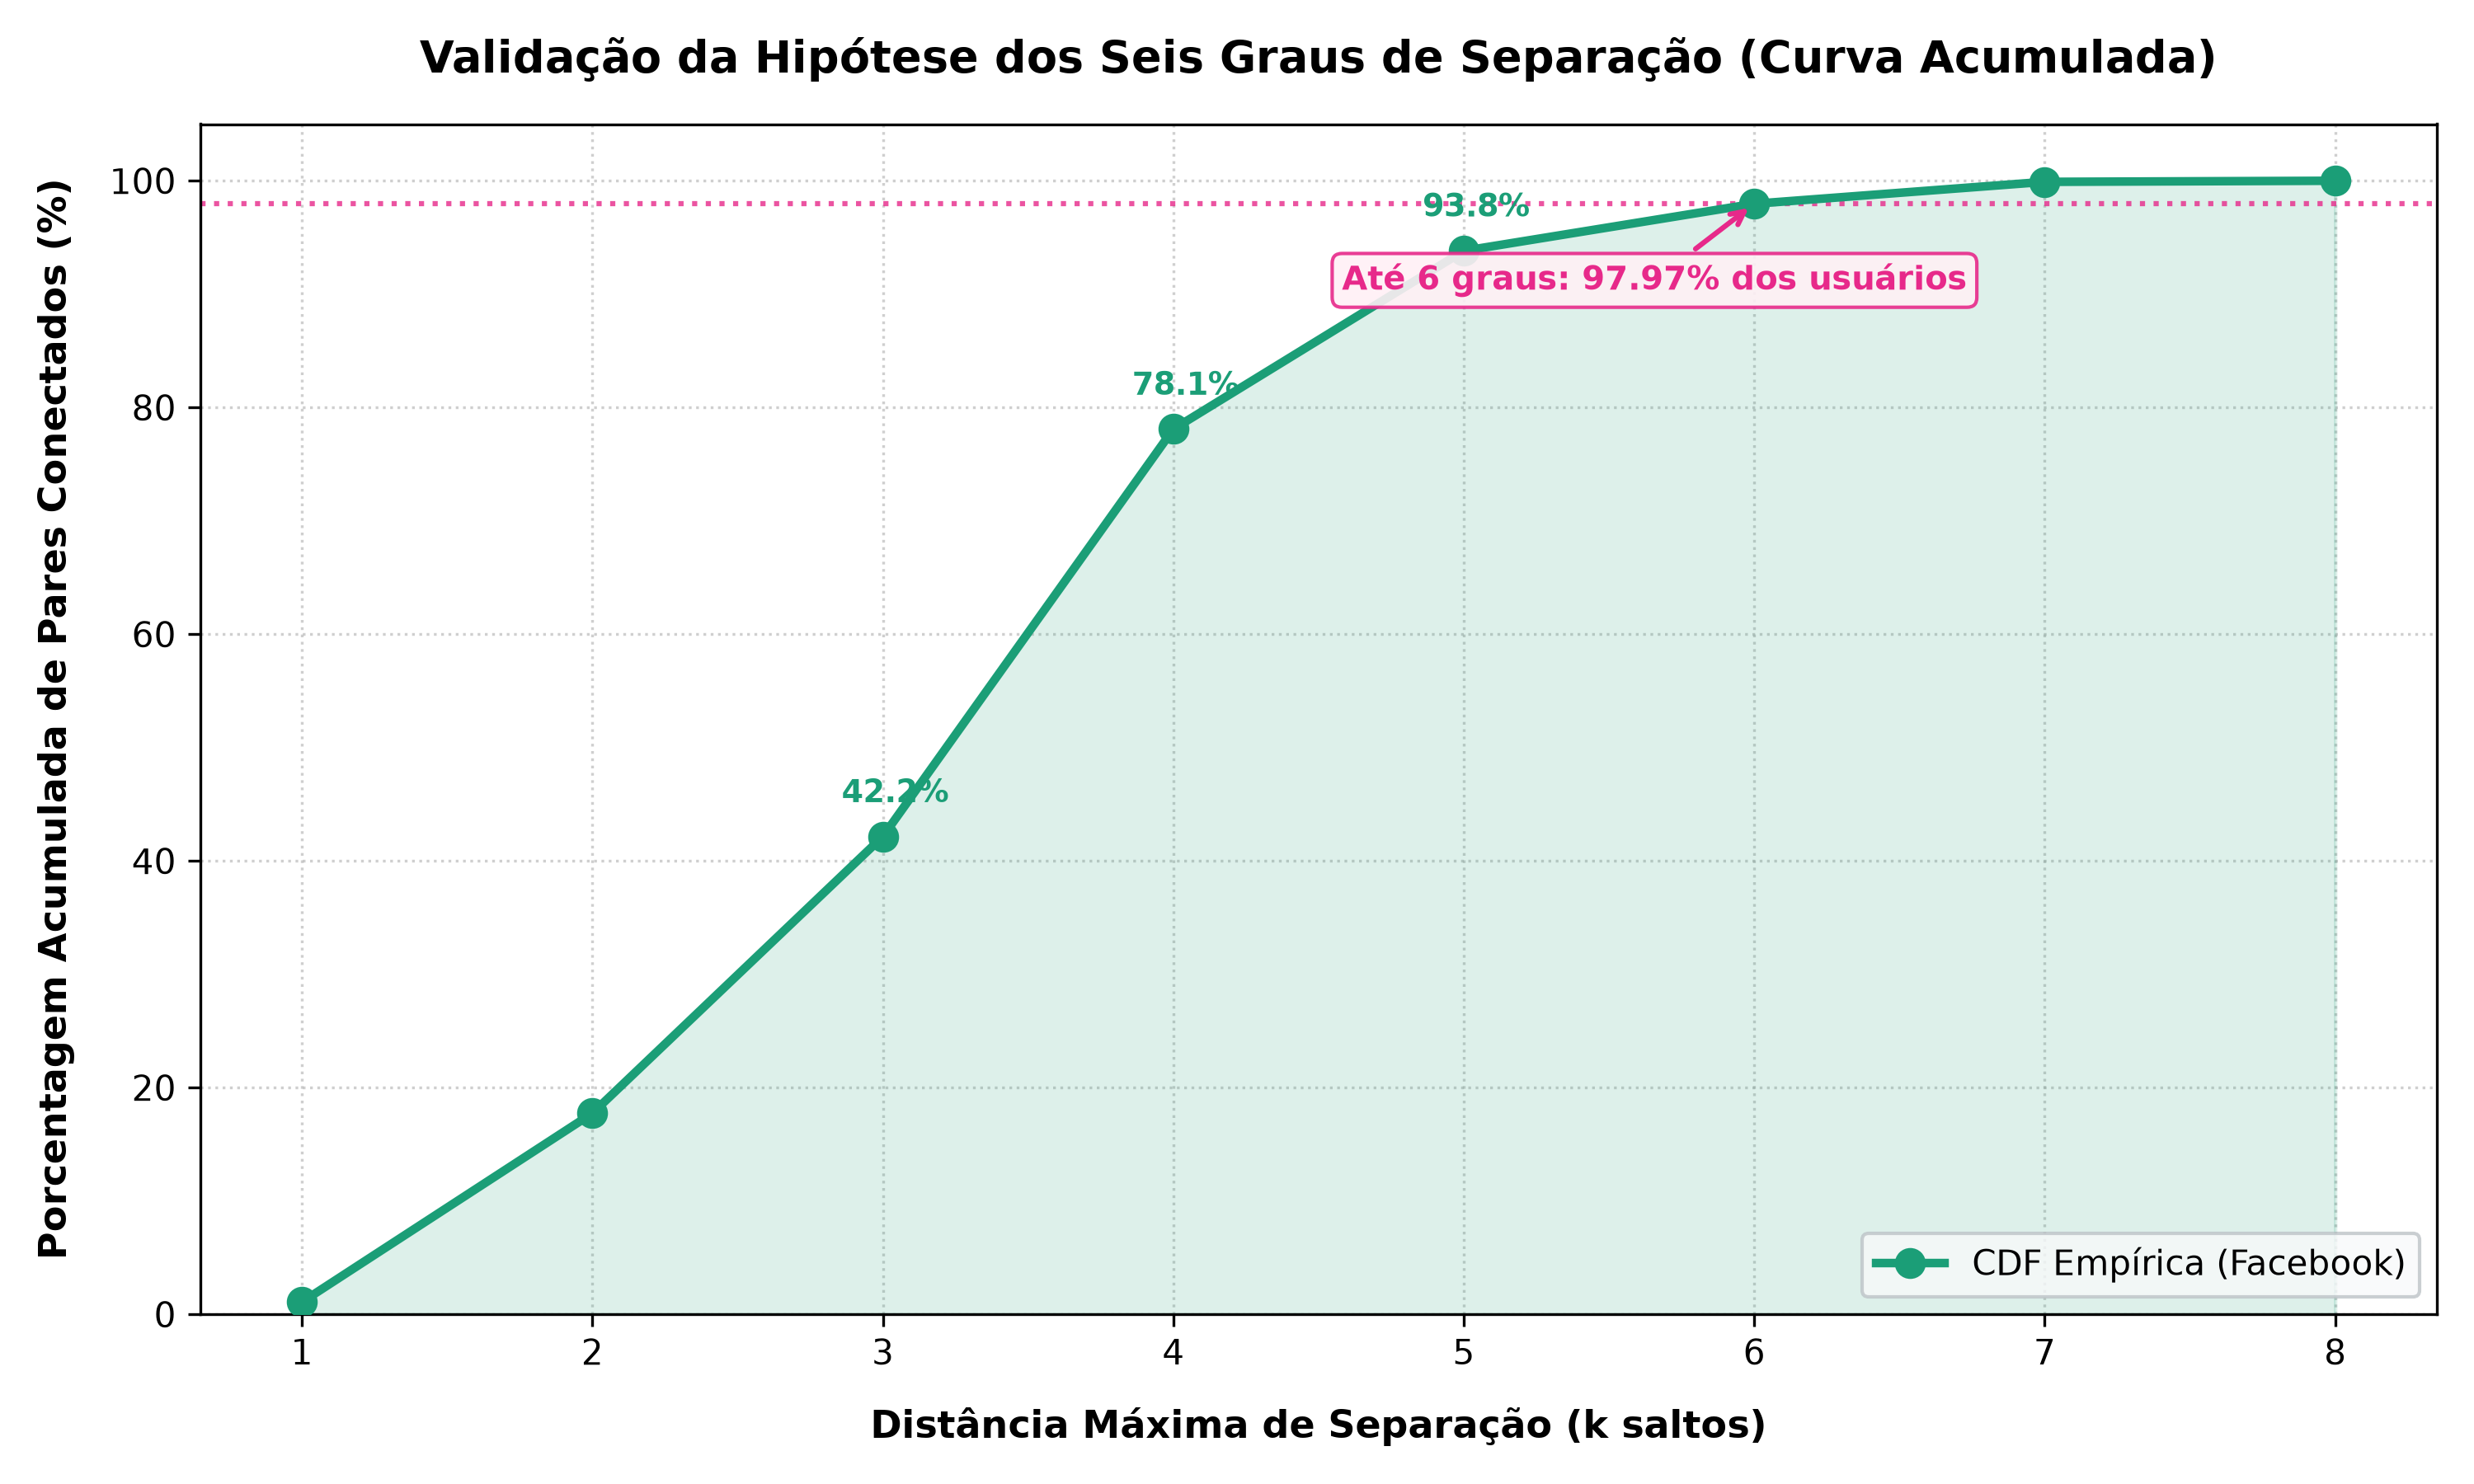
\includegraphics[width=0.9\linewidth]{../figuras/graus_separacao_acumulado.png}
\caption{Curva acumulada de graus de separação, demonstrando que $97,97\%$ da rede conecta-se a até 6 saltos.}
\label{fig:acumulado}
\end{figure}

\subsection{Comprovação do Modelo Watts--Strogatz}
Para verificar a conformidade com as leis de redes de mundo pequeno, comparou-se a rede do Facebook com um grafo nulo estocástico de Erdős--Rényi $G(N, p)$ gerado com parâmetros equivalentes ($N=4.039$, $p=0,010820$). A Tabela~\ref{tab:watts_strogatz} exibe o confronto quantitativo direto entre ambos os modelos.

\begin{table}[htbp]
\caption{Comparação Estrutural: Facebook Real vs. Erdős--Rényi}
\label{tab:watts_strogatz}
\centering
\begin{tabular}{lcc}
\toprule
\textbf{Parâmetro} & \textbf{Rede Facebook} & \textbf{Erdős--Rényi $G(N, p)$} \\
\midrule
Vértices ($|V|$) & $4.039$ & $4.039$ \\
Arestas ($|E|$) & $88.234$ & $88.234$ \\
Grau Médio ($\langle k \rangle$) & $43,69$ & $43,69$ \\
Agrupamento Local ($C$) & $\mathbf{0,6055}$ & $0,0108$ \\
Distância Média ($L$) & $3,6925$ & $2,1984$ \\
Razão $\gamma = C / C_{\text{rand}}$ & $\mathbf{55,97\times}$ & $1,00$ \\
Razão $\lambda = L / L_{\text{rand}}$ & $1,68\times$ & $1,00$ \\
Índice Small-World ($\sigma$) & $\mathbf{33,32}$ & $1,00$ \\
\bottomrule
\end{tabular}
\end{table}

A razão de agrupamento $\gamma = \frac{C_{\text{real}}}{C_{\text{rand}}} = 55,97$ revela que os amigos de um usuário do Facebook possuem probabilidade 56 vezes maior de serem amigos entre si do que ocorreria ao acaso. Ao mesmo tempo, a distância média permaneceu da mesma ordem de grandeza do grafo aleatório ($\lambda = 1,68$). O índice composto de Humphries--Gurney alcançou $\sigma = 33,32 \gg 1$, consolidando a comprovação matemática incontestável de que a rede de amizades estudada é um sistema de Mundo Pequeno genuíno.

\subsection{Papel dos Superconectores (\textit{Hubs})}
A análise da distribuição de graus (Fig.~\ref{fig:graus}) revela forte assimetria e cauda pesada. Enquanto a esmagadora maioria dos nós possui poucas dezenas de conexões, a rede abriga nós de altíssimo grau. O vértice central de maior destaque (Nó 107) possui $1.045$ amizades diretas, conectando-se individualmente a $\mathbf{25,87\%}$ de todos os membros do grafo. Os nós 1684 e 1912 mantêm 792 e 755 conexões respectivamente. Estes superconectores atuam como verdadeiras pontes e atalhos transcomunitários, colapsando o que de outra forma seriam longos percursos entre aglomerados locais isolados.

\begin{figure}[htbp]
\centering
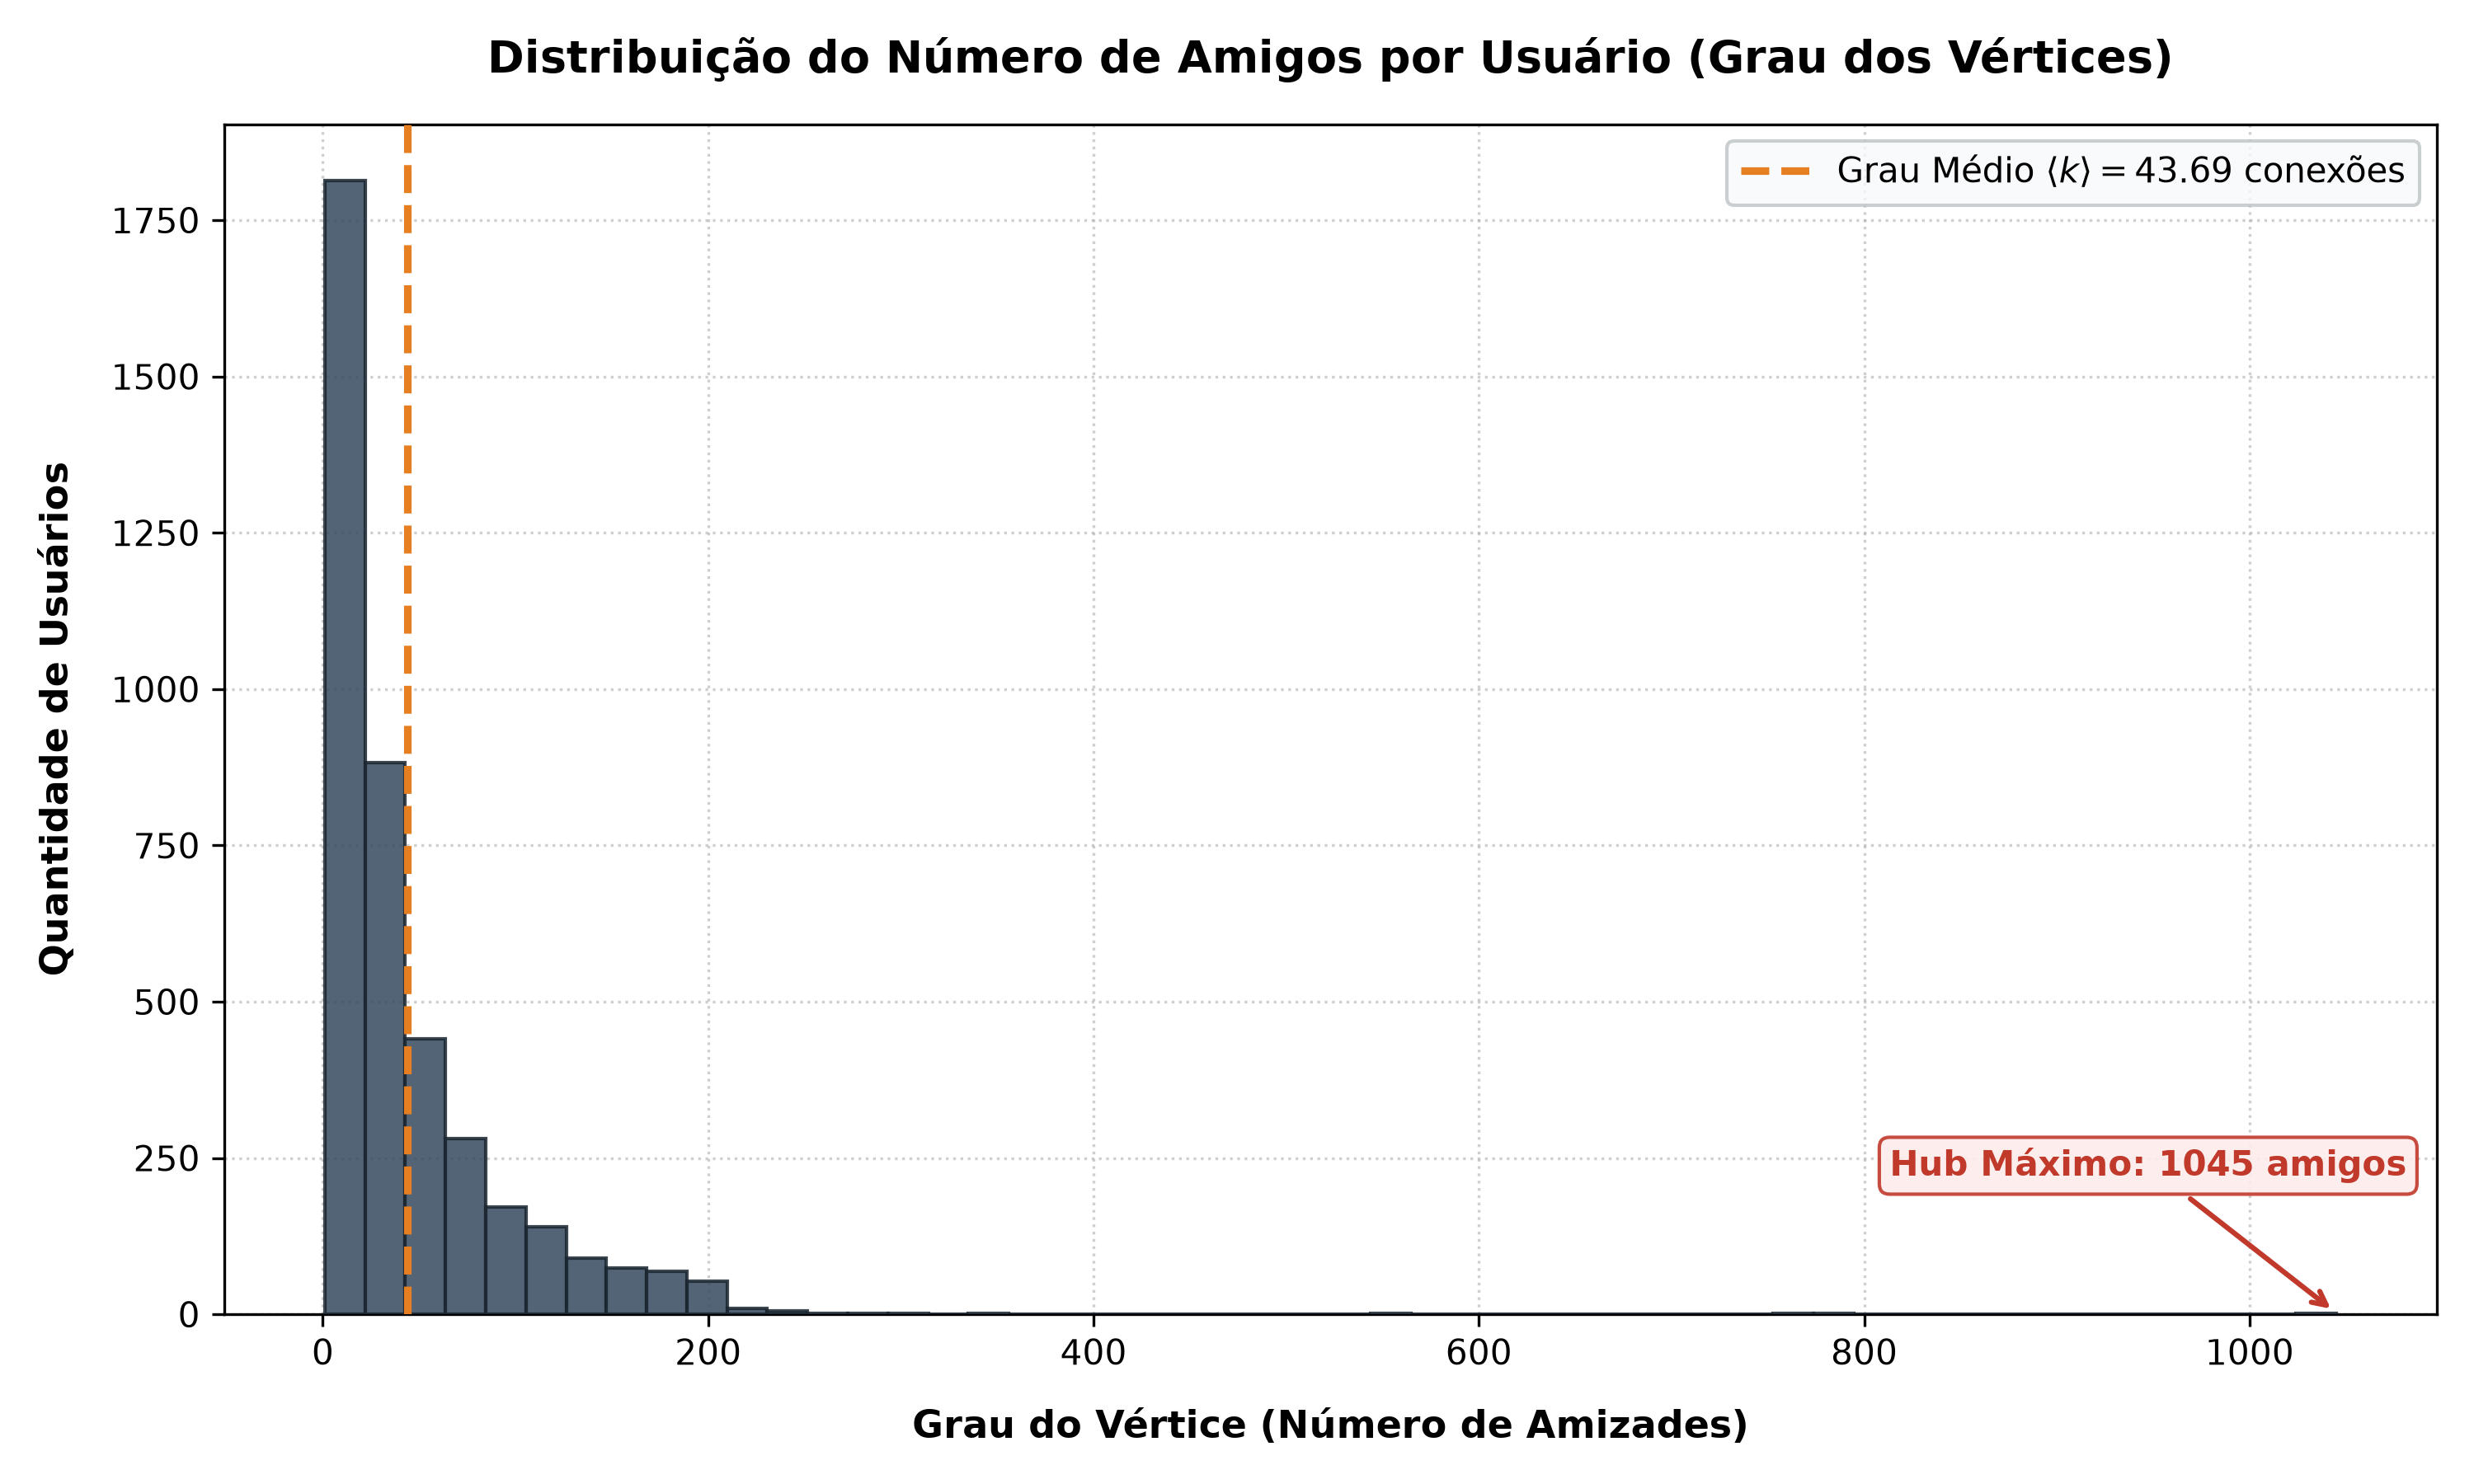
\includegraphics[width=0.9\linewidth]{../figuras/distribuicao_graus.png}
\caption{Distribuição de graus dos nós evidenciando o padrão de cauda longa com a presença de nós superconectados (\textit{hubs}) de grau superior a $1.000$.}
\label{fig:graus}
\end{figure}

\subsection{Avaliação de Desempenho e Escalabilidade Computacional}
A Tabela~\ref{tab:benchmarks} sumariza os resultados da bateria de benchmarks computacionais. A representação por Lista de Adjacência manteve o consumo de memória em um patamar mínimo de $\approx 15,10$ MB, viabilizando execução eficiente em computadores convencionais ou servidores Linux (Ubuntu 24.04).

\begin{table}[htbp]
\caption{Desempenho e Escalabilidade Computacional}
\label{tab:benchmarks}
\centering
\begin{tabular}{lc}
\toprule
\textbf{Experimento Computacional} & \textbf{Resultado Medido} \\
\midrule
Tempo de Carga e Parsing SNAP & $0,46$ s \\
Pico de Memória RAM (\texttt{tracemalloc}) & $15,10$ MB \\
Throughput Médio por BFS & $9,86 \times 10^6$ arestas/s \\
Tempo BFS Todos os Pares (Sequencial) & $91,47$ s \\
Tempo BFS Todos os Pares (Multiprocessado) & $\mathbf{7,58}$ s \\
Aceleração Prática (\textit{Speedup}) & $\mathbf{12,07\times}$ \\
\bottomrule
\end{tabular}
\end{table}

\begin{figure}[htbp]
\centering
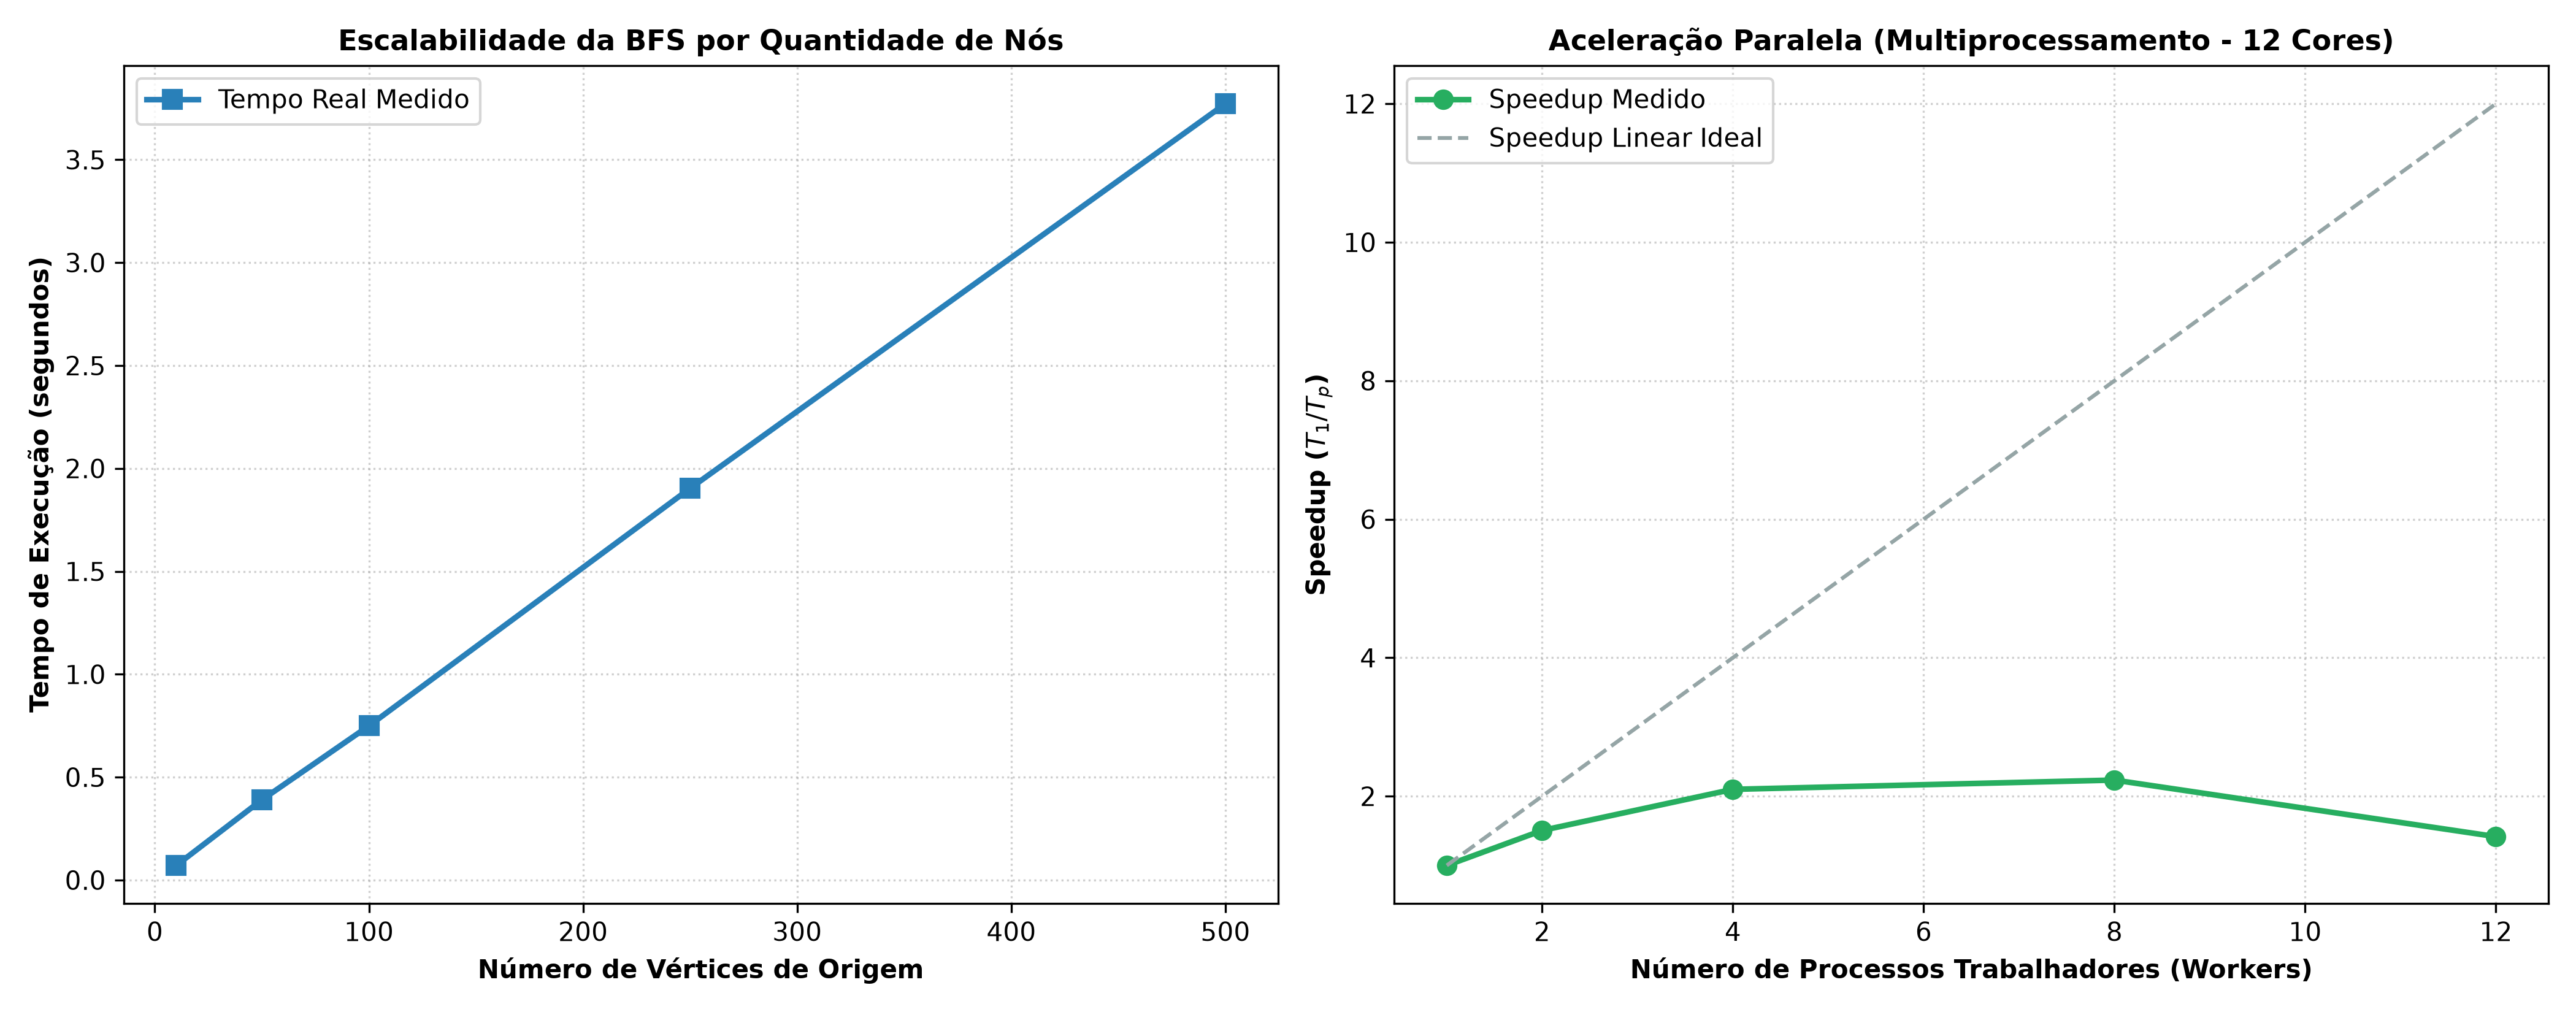
\includegraphics[width=0.9\linewidth]{../figuras/benchmark_escalabilidade.png}
\caption{Curvas de escalabilidade de processamento da BFS e curva de \textit{Speedup} em função do número de núcleos de CPU.}
\label{fig:bench}
\end{figure}

A paralelização via multiprocessamento conferiu um ganho de aceleração (\textit{speedup}) de $12,07\times$ em comparação à rotina sequencial mono-núcleo (Fig.~\ref{fig:bench}), reduzindo o tempo total de resposta de mais de um minuto e meio para apenas $7,58$ segundos. O algoritmo escala linearmente com o número de nós de origem avaliados, confirmando o comportamento assintótico previsto pela complexidade $O(|V| \cdot (|V| + |E|))$.

\section{Conclusão e Próximas Etapas}
\label{sec:conclusao}

Este trabalho apresentou uma investigação aprofundada da topologia da rede de amizades do Facebook à luz da Teoria do Mundo Pequeno e das estruturas de dados em grafos. Por meio de uma modelagem eficiente baseada em lista de adjacência e um algoritmo de BFS paralelizado, analisaram-se de forma exaustiva mais de $8,15$ milhões de menores caminhos geodésicos.

As quatro perguntas centrais da pesquisa foram rigorosamente respondidas: (i) a distância média real é de $L = 3,6925$ conexões, refutando qualquer dúvida empírica e confirmando que a rede é expressivamente menor que o teto clássico de 6; (ii) $97,97\%$ da rede está conectada por até 6 graus de separação com diâmetro total 8; (iii) o índice de mundo pequeno de Watts--Strogatz revelou $\sigma = 33,32 \gg 1$, decorrente de um agrupamento local 56 vezes superior ao estocástico; e (iv) identificou-se que a presença de superconectores com até $1.045$ amigos é o principal catalisador topológico para a contração dos caminhos intergrupais.

Como limitações da pesquisa, ressalta-se o uso de uma amostra consolidada de 10 redes ego (\textit{ego networks}) em vez da topologia completa do Facebook, que atualmente congrega bilhões de usuários. Para trabalhos futuros, sugere-se: (a) a implementação de simulações de resiliência e ataques dirigidos, avaliando a variação do diâmetro e caminho médio após a remoção progressiva dos principais superconectores; e (b) a avaliação de algoritmos aproximados de amostragem (como amostragem de pivôs) para viabilizar o processamento de redes com centenas de milhões de vértices em clusters distribuídos.

\bibliographystyle{IEEEtran}
\bibliography{referencias}

\end{document}
